We have speed-torque characteristics of a BLDC motor \cite{crowder2019electric}:
%===
\begin{align}
    T_e &= K_T I = K_T \frac{(V_s - E)}{R} = \frac{K_T}{R} (V_s - K_v \omega)
\end{align}
Where,
\begin{align*}
    \small
    \omega &- \text{\small Mechanical RPM} & &
    T_e      - \text{\small Electromagnetic torque}\\
    E        &- \text{\small Back emf} & &
    V_s      - \text{\small Supply voltage}\\
    I        &- \text{\small DC current}& &
    R        - \text{\small Terminal phase resistance}\\
    K_T      &- \text{\small Motor torque constant} & &
    K_v      - \text{\small Motor Kv value $(=K_T)$}
\end{align*}
%===
Let, $K_r = \frac{K_T}{R}$.
From (\ref{eqn::esc_input}), we have the electromagnetic torque as a function
of input and rpm:
\begin{align}\label{eqn::Te}
    T_e &= u K_r V_{in} - K_r K_v \omega
\end{align}
%===
We use the following quadratic relationship between propeller aerodynamic forces
and RPM \cite{pounds2010modelling}:
\begin{align}
    &\text{Propeller Thrust:}\quad
    F_T = C_{T} \omega^2\\
    &\text{Propeller moment due to drag:}\quad
    M_D = C_{D} \omega^2
\end{align}
%===
In our system, with the motor operating in a single direction, we consider
Coulomb friction as $M_f$ and damping due to viscous friction as $b_f\omega$.
We have the dynamic model of the BLDC motor with propeller using moment balance:
%===
\begin{align}
    J \dot \omega &= T_e - b_f \omega - M_f - C_D \omega^2
\end{align}
Where, $J$ is the moment of inertia. Also, let $b_m = b_f + K_rK_v$. We have the dynamic model:
\begin{equation}\label{eqn:dyn_mdl}
    J\dot \omega + b_m \omega + C_D \omega^2 + M_f = u K_r V_{in}
\end{equation}
%===
\subsection{Normalized Angular Velocity Input}
In the steady-state condition ($\dot \omega = 0$), (\ref{eqn:dyn_mdl}) simplifies to:
%===
\begin{align}
    &\frac{b_m}{K_r} \left(\frac{\omega_m}{V_{in}}\right) + \frac{V_{in}}{K_r} C_D \lr{\frac{\omega}{V_{in}}}^2 + \frac{M_f}{K_r V_{in}} = u
\end{align}
%===
We introduce a term, $u_{\omega}$, which represents the angular velocity of the motor with the propeller at unit supply voltage for the given PWM input ($u_p$). This is termed as "\textit{Normalized Angular Velocity}".
%===
\begin{align}
    u_{\omega} &= \frac{\omega}{V_{in}} \text{  at  } u = g_u(u_p) \\
    \implies u &= \underbrace{\frac{b_m}{K_r} u_\omega + \frac{\hat V_{in}}{K_r} C_D u_\omega^2 + \frac{M_f}{K_r  \hat V_{in}}}_{g_\omega (u_\omega, \hat V_{in})}
     \label{eqn::input_def}
\end{align}
where $\hat V_{in}$ is the battery voltage at calibration $(15.54\,V)$.
%===
The relationship between $u_\omega$ and $u_p$ can be estimated from the static
measurement data (Fig.-\ref{fig::norm_omega}).
%===
\begin{figure}[h]
    \centering
    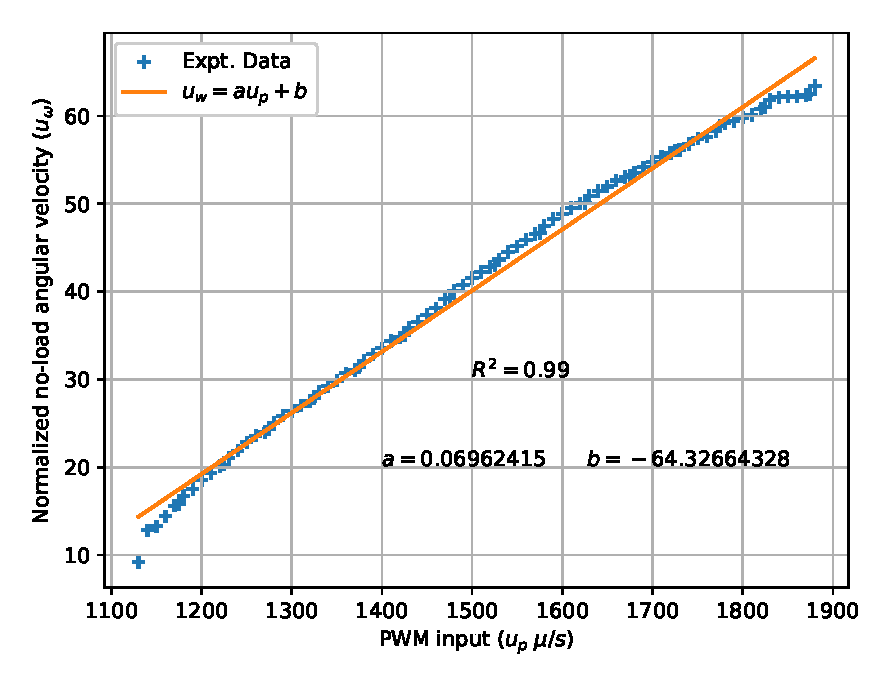
\includegraphics[width = 0.7\textwidth]{Part2/figs/3_figs/norm_omega/no-load_rpm.eps}
    \caption{$u_\omega$ as a function of $u_p$}
    \label{fig::norm_omega}
\end{figure}
%===
\begin{align}
    &u_\omega = a u_p + b
    \quad a = 0.0696
    \quad b = -64.3266\\
    \implies& g_u(u_p) = g_\omega(a u_p  + b, \hat V_{in})
    \; [\because u = g_\omega(u_\omega, \hat V_{in})]
\end{align}

\subsection{Input-Output Model}
Incorporating the input definition (\ref{eqn::input_def}) into the BLDC motor with the propeller model (\ref{eqn:dyn_mdl}), we have:
%===
\begin{equation}
    J \dot \omega + b_m \omega + C_D \omega^2 + M_f \lr{1 - \frac{V_{in}}{\hat V_{in}}} = V_{in} b_m u_\omega
            + V_{in} \hat V_{in} C_D u_\omega^2
\end{equation}
%===
We assume that the battery voltage remains approximately constant with small variations, which can be introduced as uncertainties:
%===
\begin{align}
    \hat V_{in} &= V_{in} ( 1 + \delta v)
    %\implies \frac{V_{in}}{\hat V_{in}} = 1 - \delta v\\
    \implies \lr{1 - \frac{V_{in}}{\hat V_{in}}} = \delta v
\end{align}
%====
This leads us to the following nonlinear input-output model with uncertainties:
\begin{equation}\label{eqn::nl_model}
        J \dot \omega + b_m \omega + C_D \omega^2 + M_f \delta v = V_{in} b_m u_\omega
                + V_{in}^2 (1 + \delta v) C_D u_\omega^2
\end{equation}
%===============================================================================

% ==============================================================================
\subsection{Small Perturbation Model}
Utilizing small perturbations and neglecting the gain variation $(\delta v)$, we derive the linearized model, resulting in the transfer function:
\begin{align}
    \frac{\delta \omega(s)}{\delta u_\omega (s)} &= \frac{V_{in} b_m + 2V_{in}^2 C_D u_{\omega_0}}{Js + (b_m + 2 C_D \omega_0)}
\end{align}
Additionally, we establish the following relationship between the nominal input and outputs from the input definition:
\begin{align}
    \omega_0 &= V_{in} u_{\omega_0}
    \implies \frac{\delta \omega(s)}{\delta u_\omega (s)} =\frac{V_{in} \lr{b_m + 2C_D \omega_0}}{Js + (b_m + 2 C_D \omega_0)}
\end{align}
Comparing with the standard first order model $\lr{\frac{K_m}{\tau_m s + 1}}$,
we have:
\begin{align}
    K_m &= V_{in}, \qquad
    \tau_m = \frac{J}{b_m + 2 C_D \omega_0}
\end{align}
\begin{align}
    \implies \omega_m &= \frac{1}{J}\lr{b_m + 2 C_D \omega_0}
\end{align}
Hence, the cutoff frequency is directly proportional to the nominal rpm, and the
static gain solely depends on the battery voltage.

